%%% Longer Version
% \begin{frame}[c]
% \frametitle{A Theory of Onset Temperature in 2D: Numerical Results} %$J_\sigma$

% \onslide<1->{\begin{table}[h]
% \begin{tabular}{lccccc}
% \hline\hline
% Glass Former  & Observed$^\ddagger$ $T_\mathrm{o}$  & Predicted (Approximate$^\dagger$) $T_\mathrm{KT}^\mathrm{app}$ & Predicted (RG) $T_\mathrm{KT}$  \\ \hline
% Poly-(12,0), ($\varepsilon=0.2$)  & \tikzmark{start} 0.25  & 0.38 & 0.27 \tikzmark{end}  \\
% Poly-(12,6), ($\varepsilon=0.2$)    & 0.17  & 0.16 & 0.11   \\
% Poly-(18,0), ($\varepsilon=0.0$)    & 1.10  & 2.00 & 1.40   \\
% Poly-(18,0), ($\varepsilon=0.2$)    & 0.39  & 0.51 & 0.35   \\
% Poly-(10,6), ($\varepsilon=0.1$)    & 0.17  & 0.35 & 0.24  \\
% Poly-(10,6), ($\varepsilon=0.2$)    & 0.14  & 0.15 & 0.10   \\
% \hline\hline
% \only<3->{\begin{tikzpicture}[overlay,remember picture]
%   \draw[red, thick] ([shift={(-1ex,2ex)}]pic cs:start) rectangle ([shift={(1ex,-0.5ex)}]pic cs:end);
% \end{tikzpicture}
% }
% \end{tabular}
% \vspace{-12pt}
% \caption{\footnotesize $^\ddagger$ From fitting relaxation time $\tau_\mathrm{eq}$ data. (Fraggedakis, Hasyim, Mandadapu, \texttt{arXiv:2204.07528}, 2022). $^\dagger$ From energy-entropy arguments $\beta \tilde{Y}^\mathrm{IS} d_\mathrm{c}^2 = 16\pi$.}
% %\end{ruledtabular}
% \end{table}
% }
% \vspace{-12pt}
% \begin{itemize}
%     \item<2-> Reasonable agreement is found between observed onset and RG calculation, across all polydisperse glass formers!
%     \item<4-> Prediction based on energy-entropy argument overestimates the true onset temperature $T_\mathrm{o}$
%     %\item<6-> \textbf{Finite-size effects}: MSD scales as $\ln R$ (in 2D), $R$ is the linear system size.
% \end{itemize}

% \onslide<5->{\km{\large{What are the consequences of the KT transition to dynamics at intermediate timescales?}}}

% \end{frame}


%%% Shorter Version
\begin{frame}[c]
\frametitle{A Theory of Onset Temperature in 2D: Numerical Results} %$J_\sigma$

\begin{columns}

\begin{column}{0.55\linewidth}

\onslide<5->{\begin{table}[h]
\begin{tabular}{lccccc}
\hline\hline
Glass Former  & Observed$^\ddagger$ $T_\mathrm{o}$  & RG $T_\mathrm{KT}$  \\ \hline
Poly-(12,0), ($\varepsilon=0.2$)  & \tikzmark{start} 0.25  & 0.27 \tikzmark{end}  \\
Poly-(12,6), ($\varepsilon=0.2$)    & 0.17  & 0.11   \\
Poly-(18,0), ($\varepsilon=0.0$)    & 1.10  & 1.40   \\
Poly-(18,0), ($\varepsilon=0.2$)    & 0.39  & 0.35   \\
Poly-(10,6), ($\varepsilon=0.1$)    & 0.17  & 0.24  \\
Poly-(10,6), ($\varepsilon=0.2$)    & 0.14  & 0.10   \\
2D Kob-Andersen 65:35 & 1.00 & 0.95 \\
\hline\hline
\only<6->{\begin{tikzpicture}[overlay,remember picture]
  \draw[red, thick] ([shift={(-1ex,2ex)}]pic cs:start) rectangle ([shift={(1ex,-0.5ex)}]pic cs:end);
\end{tikzpicture}
}
\end{tabular}
\vspace{-12pt}
\caption{\footnotesize $^\ddagger$ From fitting relaxation time $\tau_\mathrm{eq}$ data (Fraggedakis, Hasyim, Mandadapu, \texttt{arXiv:2204.07528}, 2022). }%$^\dagger$ Using RG calculations. (Fraggedakis, Hasyim, Mandadapu, \texttt{arXiv:2204.07528}, 2022)}
%\end{ruledtabular}
\end{table}
}
\vspace{-12pt}
\begin{itemize}
    \item<1-> There's no closed-form formula for $T_\mathrm{KT}$! 
    \item<4-> Use renormalization group (RG)\footnotemark + elastic and structural properties as input (just like $J_\sigma$).
    %\item<6-> \textbf{Finite-size effects}: MSD scales as $\ln R$ (in 2D), $R$ is the linear system size.
\end{itemize}

\end{column}

\begin{column}{0.45\linewidth}

\begin{overprint}
\onslide<2>\begin{figure}
\vspace{30pt}
$$ \frac{1}{\tilde{Y}^{\mathrm{R}} }= \underbrace{\frac{1}{\tilde{Y}^{\mathrm{IS}}}}_{\substack{\text{Bare shear} \\ \text{modulus}}}+\underbrace{\frac{A_{0}}{d_{\mathrm{c}}^{2}}\left(\left\langle\hat{\epsilon}_{i j}^{\mathrm{e}} \hat{\epsilon}_{i j}^{\mathrm{e}}\right\rangle-\frac{1}{2}\left\langle\hat{\epsilon}_{i i}^{\mathrm{e}} \hat{\epsilon}_{k k}^{\mathrm{e}}\right\rangle\right)}_{\substack{\text{Renormalization due to} \\ \text{dipolar excitations}}} $$
where $\tilde{Y}^\mathrm{R} = \beta Y^\mathrm{R} d_\mathrm{c}^2$ and $\tilde{Y}^\mathrm{IS} = \beta Y^\mathrm{IS} d_\mathrm{c}^2$

\caption{The task entails computing ensemble averages over excitation DOFs.} 

    
\end{figure}

\onslide<3>\begin{figure}
\centering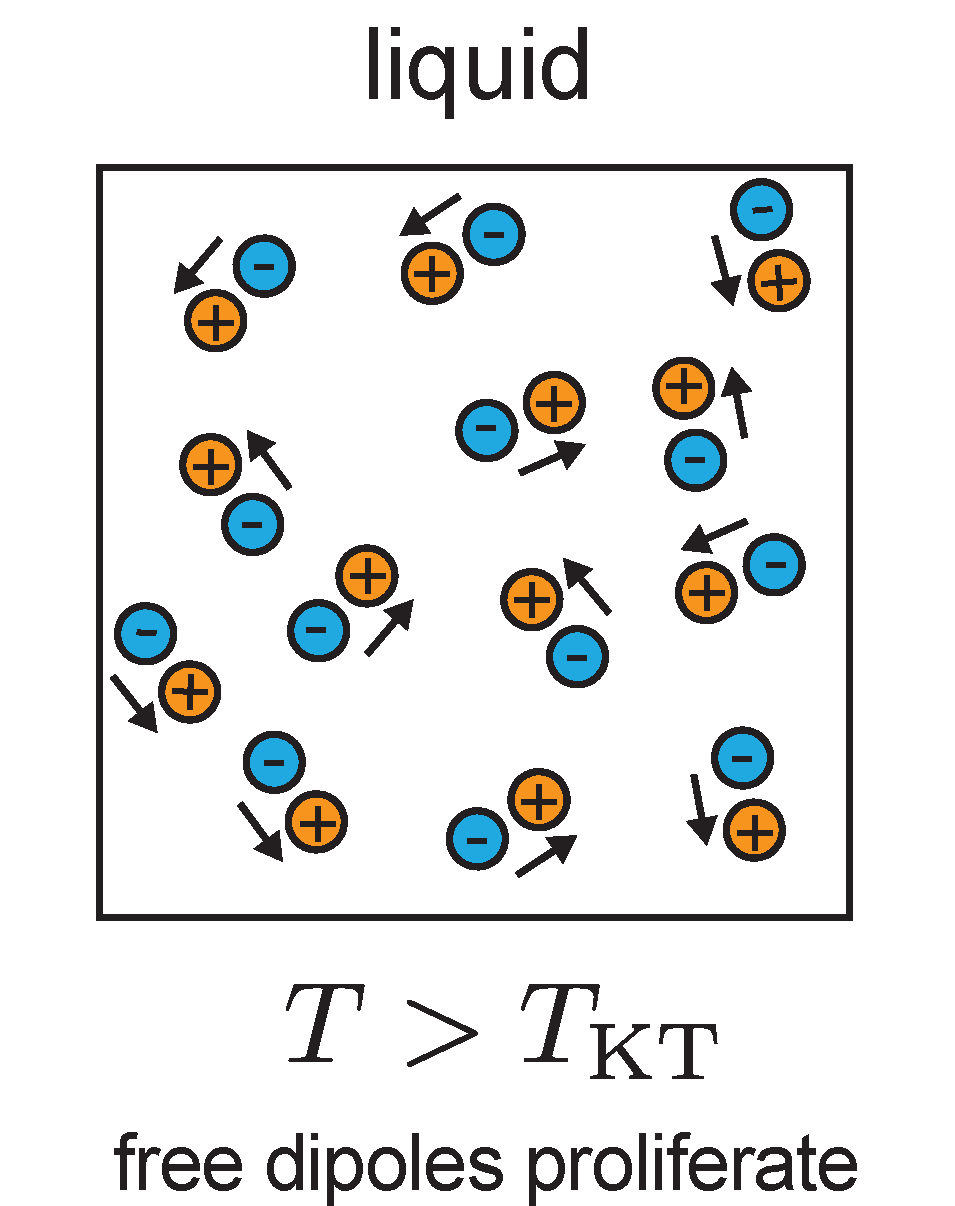
\includegraphics[height=0.675\textheight]{c.8-kt_results_1/new-mechanism-0.pdf}\caption{Melting transition is a \textbf{critical point} $\to$ naive calculations of $Y^\mathrm{R}$ fails (divergent)!}
\end{figure}

\onslide<4->\begin{figure}
\vspace{30pt}
\begin{gather*}
\frac{\mathrm{d} \tilde{Y}^{-1}}{\mathrm{~d} \ell} =\frac{\pi^{2}}{4} \tilde{y}^{2} e^{\frac{\tilde{Y}}{8 \pi}}\left(2 I_{0}\left(\frac{\tilde{Y}}{8 \pi}\right)-I_{1}\left(\frac{\tilde{Y}}{8 \pi}\right)\right) 
\\
\frac{\mathrm{d} \tilde{y}}{\mathrm{~d} \ell} =\left(2-\frac{\tilde{Y}}{8 \pi}\right) \tilde{y}+2 \pi \tilde{y}^{2} e^{\frac{\tilde{Y}}{16 \pi}} I_{0}\left(\frac{\tilde{Y}}{8 \pi}\right) 
\\
\tilde{Y}(0) = \tilde{Y}^\mathrm{IS}; \tilde{y}(0) = e^{-\beta E_\mathrm{c}}
\end{gather*}

where $I_n(x)$ is the $n$-th order modified Bessel function of the first kind

\caption{
RG yields differential equations for renormalized Young's modulus $\tilde{Y}$ and \km{fugacity $\tilde{y}$}.
} 

\end{figure}

\end{overprint}

\end{column}


\end{columns}

\only<4->{\footnotetext{
Nelson and Halperin, \textit{Phys. Rev. B} (1978)
}
}

\end{frame}